\section{Request Rate Allocation}\label{sec:rateall}

As shown in Fig.~\ref{fig:sys}, after having been notified of the optimal backend capacity by Clockwork, the developer will purchase a new MBaaS service plan or adjust the instance configuration on Amazon EC2  accordingly. Given the backend capacity fixed for the upcoming hour, there are three potential ways for Clockwork to conduct request scheduling for all users, as shown in Fig.~\ref{fig:sch}. 


\emph{Proxy mode}. As shown in Fig.~\ref{fig:sch}(a), users send all their requests to the cloud servers of Clockwork, which acts as a proxy to redirect these requests to the backend. Given that the backend capacity is $N$, we can simply sort all requests according to their delay tolerance, and send the top $N$ most urgent requests every minute. Nevertheless, an important concern with this approach is privacy. Users are, in general, not willing to reveal sensitive information to a third-party cloud service provider such as Clockwork. For this reason, it is better for users to send requests directly to the backend by themselves, but with scheduling instructions from Clockwork.

\emph{Tight control}. As shown in Fig.~\ref{fig:sch}(b), whenever a new request is generated, instead of sending it to Clockwork, the user informs Clockwork of the type and initiation time of the request, then waits for the permission to send the request to the backend. Similar to the proxy mode, every minute, Clockwork can simply give permissions to the top $N$ most urgent requests. Though this approach avoids the privacy issues, it is not scalable as the frequent communications between users and Clockwork may lead to an excessive amount of overhead and long latencies. 

\emph{Rate allocation}. To overcome the drawbacks of a stringent centralized control mechanism and give users more autonomy, we adopt a rate-based scheduling strategy, as shown in Fig.~\ref{fig:sch}(c). Within each minute, Clockwork periodically assigns rates to users, based on their reported request information. Users then schedule their own requests according to the allocated rates. In the remainder of this section, we derive a rate allocation strategy that is proved to be fair and Pareto-optimal.  

\begin{figure}[t]
	\center
	\hspace{-0cm}
	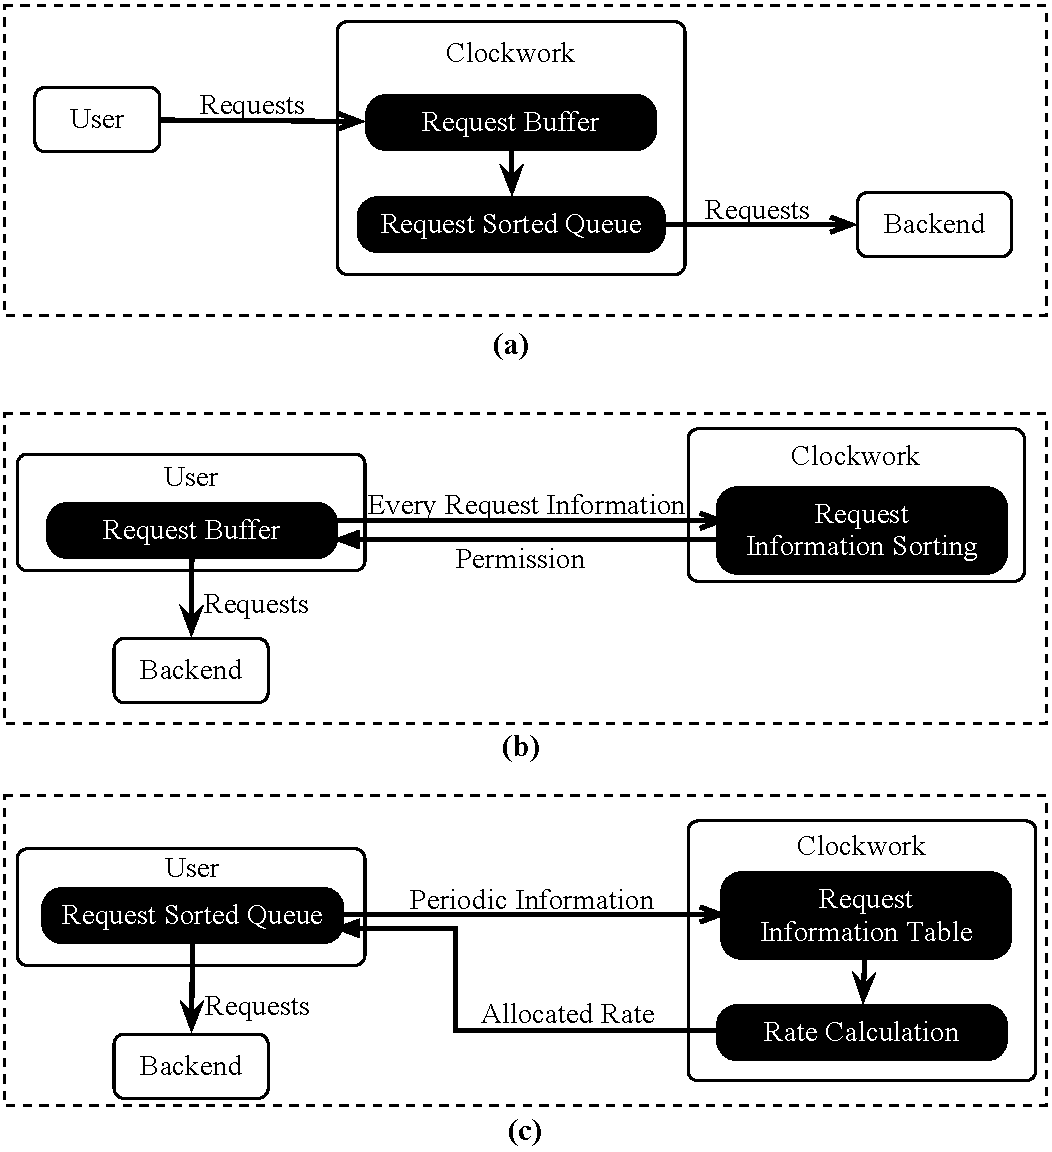
\includegraphics[width=3.2in]{figs/schedule}
	\caption{Three ways of requests scheduling.} \label{fig:sch}
	\vspace{-0.cm}
\end{figure}     

Assume that there is a finite set of $S$ users. We divide each minute into $1,2,...,T$ time slots, and users contact the cloud servers of Clockwork for a new rate at the start of each time slot. Given the backend capacity as $N$, the cap for the number of requests per time slot is $N/T$, shared by all users. At time slot $\tau$, the number of requests of user $s$ is denoted by $X_s(\tau)$, so the overall request state is $\pmb{X}(\tau)=\big(X_1(\tau), \cdots, X_S(\tau)\big)$. Clockwork allocates a rate of $R_s(\tau)$ to user $s$, the maximum number of requests that user $s$ can send within time slot $\tau$. We have $\pmb{R}(\tau) = \big(R_1(\tau),\cdots,R_S(\tau)\big)$. A rate allocation result $\pmb{R}(\tau)$ is feasible if the cap is not hit, that is, $\sum_{s=1}^{S}R_s(\tau) \le N/T$. Leveraging the definition of utility functions of the network utility maximization (NUM) problem \cite{yi2008stochastic}, we assume that the utility of assigning rate $R_s(\tau)$ to user $s$ is $X_s(\tau)\cdot U_s\big(\frac{R_s(\tau)}{X_s(\tau)}\big)$, in which $U_s(\cdot)$ is a function of $\frac{R_s(\tau)}{X_s(\tau)}$. Our objective  is to maximize the weighted sum of utilities of all users.

\begin{align}\label{equ:quota-allocation}
\vspace{-0.5cm}
\max\limits_{R_s(\tau)}~ & \sum_{s=1}^{S} \omega_s(\tau)*X_s(\tau) * U_s\big(\frac{R_s(\tau)}{X_s(\tau)}\big),\nonumber\\
	\textrm{subject to } & \sum_{s=1}^{S}R_s(\tau) \le \frac{N}{T}.
	\end{align}
in which $\omega_s(\tau)$ is the weight of user $s$, specified by the developer. The weight $\omega_s(\tau)$ is added to account for the delay tolerance of requests. If most of the requests of user $s$ are urgent, $\omega_s$ should be larger. To treat all users without bias, we adopt the same utility function for all users, i.e., $U_s(\cdot) = U(\cdot), \forall s$. Utility function $U(\cdot)$ is usually assumed to be non-decreasing and concave \cite{yi2008stochastic}. This is reasonable because a higher rate will naturally lead to a higher utility, and the increment of utility is more significant when the rate is low, but less significant when the rate is already high. We will show that, with a proper utility function $U(\cdot)$, the rate allocation result $\pmb{R}(\tau)$, as the solution to the maximization problem in (\ref{equ:quota-allocation}), can be fair and Pareto-optimal. More specifically, we choose the $\alpha$-fair utility function, widely used in the field of network resource allocation, to help achieve these ideal properties \cite{yi2008stochastic}.
	
	\begin{definition} ($\alpha$-fair function). 
		$\alpha$-fair function, introduced by Mo and Walrand \cite{mo2000fair}, is defined as:

		
		\begin{equation}\label{equ:N_w_2}
		U^{\alpha}(x) = \left\{ \begin{array}{ll}
		\frac{x^{1-\alpha}}{1-\alpha}, &\textrm{for } \alpha \in (0,\infty) \setminus \{1\},   \\
		\log x, &\textrm{for } \alpha = 1. \end{array}  \right.
		\end{equation}
		 
	\end{definition} 
	
	\begin{definition}\label{def:fairallocation}($\alpha$-fair rate allocation). 
		A feasible rate allocation result $\pmb{R}$ is called (weighted) $\alpha$-fair if, for any other feasible rate allocation result $\pmb{R}'$, we have: 
		\begin{equation}
		\sum_{s=1}^{S} w_s\frac{R'_s - R_s}{R_s^{\alpha}} \le 0. 
		\end{equation}
	\end{definition}

$\alpha$-fair rate allocation is equivalent to proportional fair rate allocation when $\alpha \rightarrow 1$, and max-min fair rate allocation when $\alpha \rightarrow \infty$. In the following context, we first give the rate allocation result according to the maximization problem in (\ref{equ:quota-allocation}) with $\alpha$-fair function, then prove that it is $\alpha$-fair and Pareto-optimal. 
	
	\begin{proposition}\label{the:rate}
		At time slot $\tau$, given the request state $\pmb{X}(\tau)$ and the cap of the number of requests  $N/T$, the rate allocation result based on $\alpha$-fair function is:
		
		\begin{equation}\label{equ:allocation}
		R_s^*(\tau) = \frac{(\omega_s(\tau))^{1/\alpha} X_s(\tau) }{\sum_{s=1}^S (\omega_s(\tau))^{1/\alpha} X_s(\tau)}\cdot\frac{N}{T}, \forall s. 
		\end{equation} 
	\end{proposition}
	
	\begin{proof}
		The Lagrangian for the problem is given by:  
		\begin{displaymath}
		L(\pmb{R}, \mu) = \sum_{s=1}^S \frac{\omega_s(\tau) X_s(\tau)}{1-\alpha}\big(\frac{R_s(\tau)}{X_s(\tau)}\big)^{1-\alpha} + \mu(\frac{N}{T}-\sum_{s=1}^S R_s(\tau)).
		\end{displaymath}
		The optimal solution corresponds to the stationary point of the Lagrangian function:
		\begin{equation}\label{equ:la}
		\begin{split}
		\frac{\partial L}{\partial R_s(\tau)} &= \omega_s(\tau)(\frac{R_s(\tau)}{X_s(\tau)})^{-\alpha} - \mu, \forall s,\\
		\frac{\partial L}{\partial \mu}& = \frac{N}{T} -\sum_{s=1}^{S} R_s(\tau).
		\end{split}
		\end{equation}
		By setting $\partial L /\partial R_s(\tau) = 0$, we have:
		\begin{equation}\label{equ:1}
		R_s(\tau) = X_s(\tau) (\frac{\mu}{\omega_s(\tau)})^{-\frac{1}{\alpha}}, \forall s.
		\end{equation}
		By setting $\partial L /\partial \mu = 0$, we have:
		\begin{equation}\label{equ:2}
		\sum_{s=1}^SR_s(\tau) = \frac{N}{T} = \sum_{s=1}^SX_s(\tau) (\frac{\mu}{\omega_s(\tau)})^{-\frac{1}{\alpha}}.
		\end{equation}
		Combining (\ref{equ:1}) and (\ref{equ:2}), we can get the rate allocation result as (\ref{equ:allocation}). 
	\end{proof}
	
	\begin{theorem}
		The rate allocation result given by Proposition \ref{the:rate} is weighted $\alpha$-fair.  
	\end{theorem}
	
	\begin{proof}
    Let $\pmb{R}(\tau) \ne \pmb{R}^*(\tau)$ denote an arbitrary feasible rate allocation result. Multiplying  (\ref{equ:1}) by $(R_s(\tau) - R_s^*(\tau))$, we have:
    \begin{displaymath}
    \big(R_s(\tau) - R_s^*(\tau)\big)\omega_s(\tau) \big(\frac{R_s^*(\tau)}{X_s(\tau)}\big)^{-\alpha} = \mu \big(R_s(\tau) - R_s^*(\tau)\big).
    \end{displaymath} 
    Summing over all $s$, we have:
    \begin{displaymath}
    \sum_{s=1}^S\omega_s(\tau) X_s(\tau)\frac{R_s(\tau) - R_s^*(\tau)}{(R_s^*(\tau))^{\alpha}}  = \mu \sum_{s=1}^S\big(R_s(\tau) - R_s^*(\tau)\big).
    \end{displaymath} 
     According to (\ref{equ:la}), we have $\sum_{s=1}^{S} R_s^*(\tau) = {N}/{T}$ and
     
     \noindent$\sum_{s=1}^{S} R_s(\tau) \le {N}/{T}$. Hence, we have:
     \begin{displaymath}
     \begin{split}
     \sum_{s=1}^S\omega_s(\tau) X_s(\tau)&\frac{R_s(\tau) - R_s^*(\tau)}{(R_s^*(\tau))^{\alpha}} = \mu \sum_{s=1}^S\big(R_s(\tau) - R_s^*(\tau)\big) \\
     &= \mu (\sum_{s = 1}^S R_s(\tau) -\sum_{s=1}^S R_s^*(\tau)) \le 0.
     \end{split}
     \end{displaymath}
     The strict inequality holds for all $\pmb{R}(\tau)\ne \pmb{R}^*(\tau)$, due to the uniqueness of $\pmb{R}^*(\tau)$. Based on definition \ref{def:fairallocation}, the rate allocation result given by (\ref{equ:allocation}) is weighted $\alpha$-fair.  
	\end{proof}
	
	The efficiency of the rate allocation result given by Theorem \ref{the:rate} is characterized by Pareto-optimality as follows. 
	
	\begin{definition}(Pareto-optimality). A rate allocation result $\pmb{R}(\tau)$ is said to be Pareto-optimal, if for any rate allocation result $\pmb{R}'(\tau)$, which satisfies $\forall s, R_s'(\tau) \ge R_s(\tau)$,  it must be true that $\pmb{R}(\tau) = \pmb{R}'(\tau)$. 
	\end{definition}
	
	Pareto-optimality implies that there is no other rate allocation result that can improve every user's utility by assigning everyone a higher rate. 
	
	\begin{theorem}
		The rate allocation result given by Proposition \ref{the:rate} is Pareto-optimal.  
	\end{theorem} 
	\begin{proof}
		Assume that there exists a feasible rate allocation result $\pmb{R}(\tau)$, which satisfies $\forall s, R_s(\tau) \ge R_s^*(\tau)$. We have:
		\begin{displaymath}
		\begin{split}
		&\sum\limits_{s=1}^S R_s(\tau) \ge \sum\limits_{s=1}^S R_s^*(\tau) \\
		&= \sum\limits_{s=1}^S\frac{(\omega_s(\tau))^{1/\alpha} X_s(\tau) }{\sum_{s=1}^S (\omega_s(\tau))^{1/\alpha} X_s(\tau)}\cdot\frac{N}{T} =\frac{N}{T}.
		\end{split}
		\end{displaymath}
		If $\pmb{R}(\tau) \ne \pmb{R}^*(\tau)$, there exists at least one user $s$, $R_s(\tau) > R_s^*(\tau)$, and the cap on the number of requests per time slot will be violated. Therefore, it must be true that $\pmb{R}(\tau) =\pmb{R}^*(\tau)$. 
	\end{proof}

  	




	
	
	
